\documentclass[border=3mm]{standalone}
\usepackage{tikz}
\usetikzlibrary{circuits.logic.US}

\begin{document}
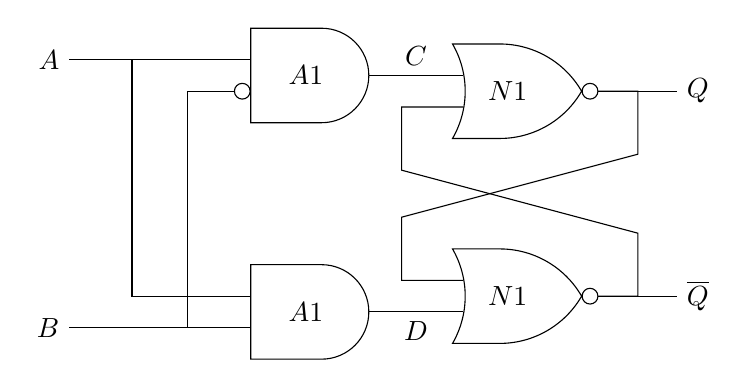
\begin{tikzpicture}[circuit logic US,
                    tiny circuit symbols,
                    every circuit symbol/.style={fill=white,draw,logic gate input sep=4mm, logic gate inverted radius=1mm}
]

% Draw the NOR gates
\node [nor gate, inputs = nn,info=center:$N1$] at (0,0) (nor1) {};
\node [nor gate, inputs = nn,info=center:$N1$] at ($(nor1.south)+(0cm,-2cm)$) (nor2) {};
\draw (nor1.input 1) ++(left:6mm) node[above] {$C$};
\draw (nor2.input 2) ++(left:6mm) node[below] {$D$};

% Draw the AND gates
\node [and gate, inputs = ni,info=center:$A1$] at ($(nor1.input 1)+(-2,0)$) (and1) {};
\node [and gate, inputs = nn,info=center:$A1$] at ($(nor2.input 2)+(-2,0)$) (and2) {};
\draw (and1.input 1) -- ++(left:23mm) node[left] (B) {$A$};
\draw (and1.input 1) ++(left:15mm) |- (and2.input 1);
\draw (and2.input 2) ++(left:8mm) |- (and1.input 2);
\draw (and2.input 2) -- ++(left:23mm) node[left] (C) {$B$};
%
%\draw (and1.output) |- (nor1.input 1);
%\draw (and2.output) |- (nor2.input 2);
%
\draw (and1.output) |- (nor1.input 1);
\draw (and2.output) |- (nor2.input 2);
\draw (nor1.output) -- ++(right:10mm) node[right] (U) {$Q$};
\draw (nor2.output) -- ++(right:10mm) node[right] (V) {$\overline{Q}$};

% Draw the NOR gate outputs back to respective inputs
\draw (nor1.output) -- ++(right:5mm) -- ++(0,-8mm) -- ++(-3.0cm,-8mm )|- (nor2.input 1);
\draw (nor2.output) -- ++(right:5mm) -- ++(0,8mm) -- ++(-3.0cm,8mm )|- (nor1.input 2);

\end{tikzpicture}
\end{document}
